\documentclass{article}
\usepackage[utf8]{inputenc}
\usepackage{graphicx}
\usepackage{amssymb, amsmath, amsthm}
\usepackage{bbm}
\usepackage{biblatex}
\addbibresource{references.bib}
\newcommand\numberthis{\addtocounter{equation}{1}\tag{\theequation}}
\usepackage[margin=1in]{geometry}
\graphicspath{ {report_figures/} }
\parskip = 0.1in

\begin{document}
\title{Forest Fires: An Analysis of the Initial Spread Index}
\date{December 12, 2017}
\maketitle
\begin{abstract}

\end{abstract}

\section{Introduction}

Forest fires ravage entire ecosystems and have lasting consequences on the environment beyond their path of destruction. These fires deplete oxygen from the atmosphere, impact the lumber industry, vanquish animal habitats, and damage areas of natural beauty. They also contribute to pollution, carbon emission, soil erosion, flooding, and water contamination. As our planet is increasingly threatened by rising temperatures and dangerous policies, it is imperative that we be more responsible with our resources. Statistics offers many tools that can reveal ways to be more mindful and efficient in addressing complex problems. Here, we will use the theory of linear modeling to analyze the initial spread of forest fires. In particular, we look to pick up where Smokey Bear left-off: the next line of defense after prevention is early-detection. By understanding the factors of initial spread, we hope to contribute to the fight against forest fires.

To accomplish this goal, we examine Initial Spread Index (ISI) as our response variable from data obtained in Monteshino Natural Park between 2000 and 2003. It is worth emphasizing that our target is not forest fire occurrences. This subtle difference goes against our intuition. For example, regarding the presence of people, we expect that the number of fires increases with the presence of people. On the other hand, more people means earlier detection. Therefore, we have no $\textit{a priori}$  knowledge of the relationship between people and ISI. This difficulty extends to other variables such as rain and wind, in which different arguments could be made to explain different possible relationship with ISI.

Our analysis takes a standard approach by first splitting our data into training and testing sets, then performing feature engineering and variable selection on our training set, fitting our various models, and finally evaluating these models on our testing set. While we do make predictions on the test set, our focus is on making statistically significant inferential conclusions. Therefore, we avoid using overly complicated transformations, and when faced with competing models, we select the simpler version. We understand that this may result in a sub-optimal predictive model, but our goal is to obtain interpretable coefficients and generalizable results. We chose this inferential approach because we believe the first step to combating forest fires is understanding how they initially spread, and without an understanding, what good is a highly predictive model? Naturally we want to understand the likely causes of forest fires with a high ISI, of which we explore variables related to climate, time, location, and people.

This paper is organized as follows. In Section \ref{Background} we give a summary of our reference paper and restate our goal in this context. In Section \ref{Analysis} we outline our analysis, including our initial exploration of the data, all feature engineering and variable selection, and our final modeling decisions. In Section \ref{Prediction}, we apply our final model to our holdout set in order to make unbiased inferences. We conclude our project in Section \ref{Discussion} with a general discussion of our results. Finally, relevant R code may be found in the attached Appendix.

\section{Background}\label{Background}

The subject of modeling forest fires has been well studied. In the reference paper provided, Paulo Cortez and Anibal Morais explored the potential of machine learning algorithms in predicting area burned by wildfires (TODO ADD CITATION). They compared support vector machines, decision trees, multiple linear regression, neural networks, random forests and a naive mean prediction with four sets of features. Cortez and Morais found that support vector machines had the overall best success in predicting area burned. Their proposed solution is an SVM using as input a combination of temperature, rain, relative humidity and wind speed.

Further, we looked into the history of the Canadian Forest Fire Weather Index (FWI). Specifically, Van Wagner 1987 (TODO ADD CITATION) details the development of and equations used in the FWI system. Van Wagner specified that $$ISI =  0.208(2^{WIND/19})(91.9e^{-.1386FFMC})(1+FFMC^{5.31}/(4.93*10^7))$$
However, in our initial assessment of this equation, we considered it cheating to use it directly in our models. Further, we consider innovation to be a goal in this paper. So we attempted not to let knowledge of the equation influence our models.

\begin{itemize}
\item how data were collected
\item goal
\item restate prediction problem

\end{itemize}
\section{Modeling \& Analysis}\label{Analysis}

\subsection{Data Overview}

ISI attempts to quantity the risk associated with the initial spread of a forest fire. Heuristically, we expect variables that describe the weather characteristics of Monteshino Natural Park as well as the terrain within the park to affect the initial spread of a newly sparked forest fire. While we do not know how ISI is calculated, we surmise that these characteristics should play a major role in our modeling procedure. While we expect that these two classes of data should be sufficient in modeling ISI, there is a third, far more subtle, factor that we need to consider. First consider Figure \ref{fig:human_factor}
\begin{figure}[h!]
\centering
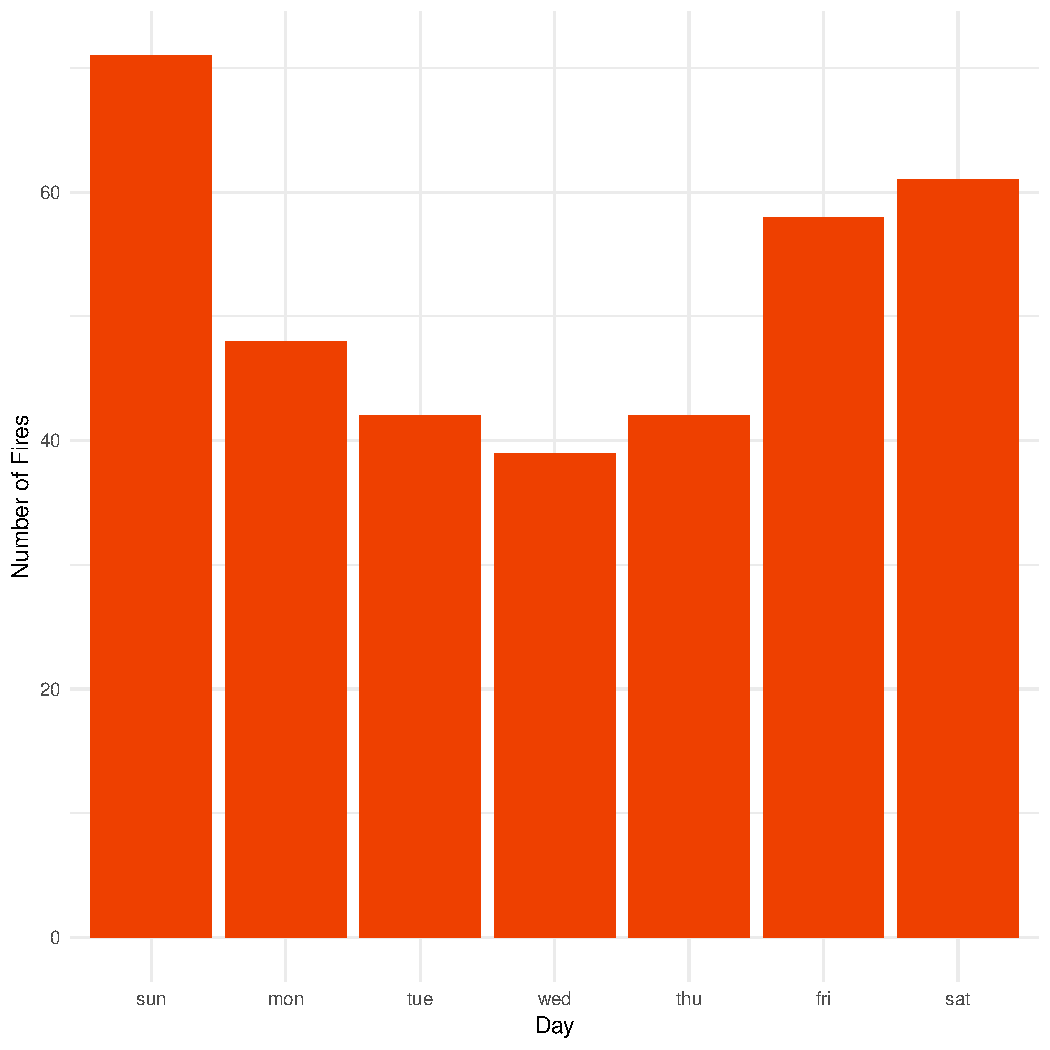
\includegraphics[width=0.45\textwidth]{day_bar.pdf}
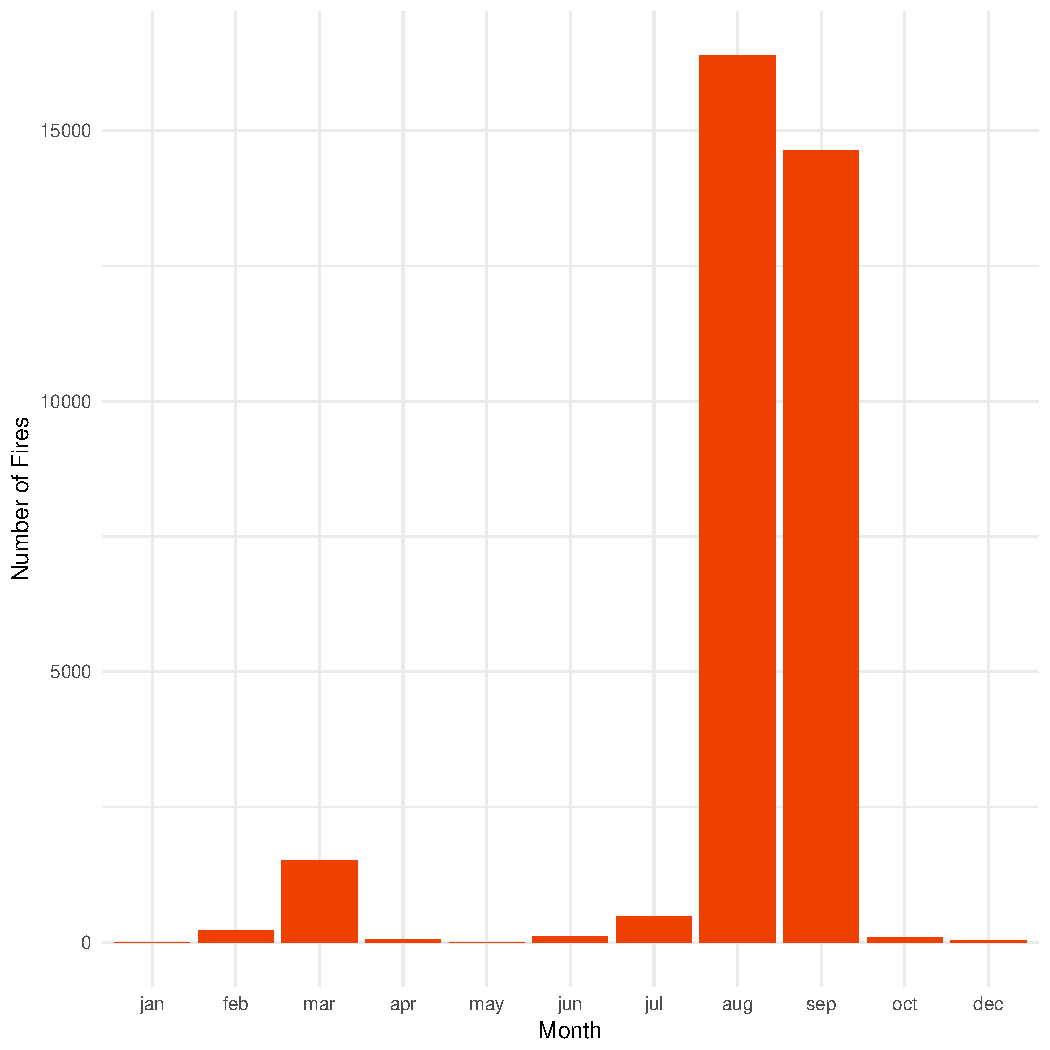
\includegraphics[width=0.45\textwidth]{month_bar.pdf}
\caption{We expect that with more fire on the weekends }
\label{fig:human_factor}{}
\end{figure}
Based on these figures, it appears that fires are far more likely to occur in late summer and on the weekends. While the abundance of fires occurring in summer may be attributable to climatic changes, we suspect that the imbalance of fires on the weekend must be connected in some way to the presence of more visitors to the park. While we do not have direct data on the number of individuals in the park on any given day, we expect that this variable greatly affects the way in which \textit{the data was collected}. It seems reasonable to assume visitors to the park were either responsible for reporting the presence of a fire or starting the fires themselves. Therefore, when more visitors are in the park, we expect the response time to a fire to decrease, and the initial spread of the fire to decrease as well. Hence, while we expect visitors to have no affect on how fast fires spread, due to the nature in which the data was collected, we include variables that model human presence.  

With this in mind, we categorize our data into three types: weather, human impact, and geospatial. Weather indicators contain information such as rain, temperature, relative humidity, and other indices such as FFMC, DMC, and DC. We attempt to capture the affect of geospatial components using the $(X,Y)$ coordinates as well as design new variables that attempt to identify homogeneous regions of the park. Lastly, we model the human impact inherent in data collection by introducing variables that serve as proxies for the number of visitors to the park on any given day. 



%\par The ISI is an index that reflects the initial spread of a fire and is calculated using the Fine Fuel Moisture Code (FFMC) and the wind speed (cite) (talk about figure?). Because of this, the FFMC and wind variables should be important predictors. Looking at the plots (add plots) of these variables against ISI, there is clearly a relationship between ISI and FFMC. The relationship is not as clear between ISI and wind speed. In addition to these variables, we also believe that there are temporal factors that affect ISI. [what do we want to say about this..? because looking at the boxplot, it seems that weekdays are actually higher in ISI]. In particular, we believe that the summer months are important because it is dryer, which allows for fires to spread easily, and people are more likely to go to the forest and may cause accidental forest fires. For the same latter reason, we believe that weekends will also be a good indicator of ISI. Furthermore, because the spread of a fire depends on the terrain of the land, it is reasonable to believe that spatial factors will have a great influence on ISI. Areas that are further away from populated areas and that have more trees should have a higher ISI because it would take a longer time for the fires to be detected and the trees will provide fuel for the fire. 

\begin{itemize}
\item initial ideas: what should matter, types of covariates (spatial, temporal, index)
\item first plots
\item identify problems (colinearity, skewness)
\end{itemize}

\subsection{Feature Design}\label{Engineering}

\begin{itemize}

\item transformations
\par
(should we add some plots) We transformed several covariate in order to get the most information out of the variables based on our intuition and on our initial look of the data set. According to Cortez and Morais (2007), the area variable was transformed using $y = ln(area + 1)$ because it is highly concentrated around zero (lower than $100m^2$ burned) and right skewed. We did the same transformation for the area variable in our data set. Similar to area, the rain variable is also concentrated around zero and right skewed. However, instead of using $\textit{ln}$, we changed the variable into an indicator of whether there was rain in order to get the most out of the few data points that were not zero. We also grouped the FFMC index into 10\% quantiles because it was left skewed and had a majority of data points that were above 80. An indicator of summer is 1 for the months of June, July, August, and September, which were chosen based on the climate of Portugal and looking at the number of data points. We created two weekend indicators -- one that includes Friday to Sunday and another that includes Friday to Monday. Monday was included because there may be some lag effects from people staying there all weekend. We determine which variable is more important during the variable selection phase. 
\item creations
\par
In addition to transforming variables, we also created several new covariates. Using temperature and relative humidity, a wetness metric (cite?) was created because it affects the fire spread. (explain more of how this is created--ask Matthew). (Not sure if we want to include this part and/or combine with Nate's geo-spatial part). We also included a forest indicator which was manually created using a map of the Monteshino Natural Park and corresponding it with the grid of coordinates provided in the data. An indicator of 1 means that the cross-section of the coordinates contains a forest area. 
\item One interesting feature class in this problem is geo-spatial. The raw data contains $X$ and $Y$ coordinates corresponding to a grid that has been overlaid on the map of Monteshino Natural Park. Each coordinate ranges from 1 to 9, therefore there are 81 total boxes in the grid. Of course, the first attempts at capturing any geo-spatial signal involved looking at the raw $X$ and $Y$ coordinates, as well as their interaction. Unfortunately, many of these boxes were sparse and the 81 degrees of freedom necessary for the raw grid were detrimental to the modeling process. Instead, we designed several features based on these values. This resulted in three candidate features. First, we created new coordinates $X2$ and $Y2$ that were created from the following algorithm
\begin{align*}
1&. \text{ sum the first row, last row, first column, last column} \\
2&. \text{ combine the row or column with the lowest sum with its neighboring row or column} \\
3&. \text{ repeat steps 1 and 2 until every box contains at least 1\% of the data}
\end{align*}
The algorithm was written under the belief that your neighbors are most similar to you and therefore should be the first candidates when grouping spaces together. Applying this algorithm, we reduced the number of boxes from 81 to 12. We note that $Y2$ only has two levels, which is unsurprising since Monteshino Natural Park is wider than it is tall. The other two engineered features integrated outside information. For these, we found a topographical map of Monteshino Natural Park on Google Maps and overlaid the original $X-Y$ grid.  The result is Picture \#\#\#. From this, we created $\textit{forest\_ind}$, which is a binary variable that takes the value 1 when the box is mostly covered in trees and 0 otherwise, and $\textit{grid\_group}$, which identifies five major mountain ranges and groups the boxes that cluster around these mountain ranges. Both of these variables are intuitively appealing, since obviously a forest fire needs trees and generally travelers hike and camp on a single mountain range.

\end{itemize}

\subsection{Variable Selection}

In order to effectively consider all variables discussed above while still making inferential statements about ISI, we use penalization schemes in order to identify important variables and classes of variables in our problem. While Ridge Regression has several nice properties, we turn to LASSO as a variable selection tool in our analysis. By using LASSO, we allow an $L_{1}$ penalty to \textit{zero-out} uninformative variables while also identifying variables that are representative of entire groups of variables. 



\begin{itemize}

\item FFMC
(we can add the chart fig 1 from the paper to show that rain, rh, temp, and wind is included in ffmc)
\item LASSO
\item tradeoff between interpretability for inference vs prediction
\item creation of competing models - with and without FFMC
\item The three engineered geo-spatial features from Section \ref{Engineering} were all considered as covariates. Unfortunately, none were selected during variable selection, as LASSO zeroed their coefficients are they were not significant under further scrutiny. However, we firmly believed that there should be signal from these geo-spatial features. Our next attempt was to fit a Mixed Model with $\textit{grid\_group}$ or $X2:Y2$ as the random intercepts. Again, this did not provide an improvement. Similarly, we tried weighting by the number of fires in $\textit{grid\_group}$ and $X2:Y2$ to no avail. We concluded that without further refinement or data collection, all of the geo-spatial signal was being picked up by the class of climate features, and therefore $X$, $Y$, and the derivative variables were discarded for our final model.

\end{itemize}

\subsection{Modeling}

\section{Prediction}\label{Prediction}

%\begin{itemize}
%\item apply best model to test set
%\item report diagnostics
%\item report p-values
%\item MSE or some loss function
%\item final inferences
%\end{itemize}

Finally, we turn our attention to  evaluating the weather only based model by using the holdout set.  We begin by fitting the chosen model for on the test set data, which comprises 30\% of the original data set. These estimates are reported in table \ref{Parameter Estimates}.  

\begin{table}
\centering
\begin{tabular}{ | l | c | c |}\hline
  Variable & Estimate & Standard Error \\ \hline
  Intercept & 1.31 & 0.24 \\
  Is Summer & 0.58 & 0.16 \\
  Wind & 0.079 & 0.029 \\
  Temperature & 0.045 & 0.012 \\
  Is Raining & -0.26 &   0.47 \\
  \hline
\end{tabular}
\caption{Final Parameter Estimates}
\label{Parameter Estimates}
\end{table}


As previously noted, the estimates from normal theory are close to the estimates from a bootstrap, so the 95\% confidence intervals are reported based assuming normal errors:
\begin{table}
\centering
\begin{tabular}{  | l | c | }\hline
  Variable & $95\%$  Confidence Interval \\ \hline
  Intercept & $(  0.84,1.79  )$ \\
  Is Summer & $( 0.26,0.90   )$\\
  Wind & $(  0.02,0.14  )$ \\
  Temperature & $(  0.02,0.07  )$ \\
  Is Raining & $(  -1.19,0.67  )$ \\
  \hline
\end{tabular}
\caption{Final Confidence Intervals}
\label{Confidence Intervals}
\end{table}
All the confidence intervals except for the binary Is Raining variable do not contain zero, so we conclude that they are all different than zero.
However, the Is Raining confidence interval does contain zero, so we do not conclude that the Is Raining variable is significantly different than zero.  We also note that the confidence interval is quite wide and there is a large standard error because there were only two data points with rain in the test set. While rain was uncommon in the training set, it was less sparse than in the test set, so it is difficult to make inference on such a variable. 
%Fix Up Graphics Path
\begin{figure}
\centering
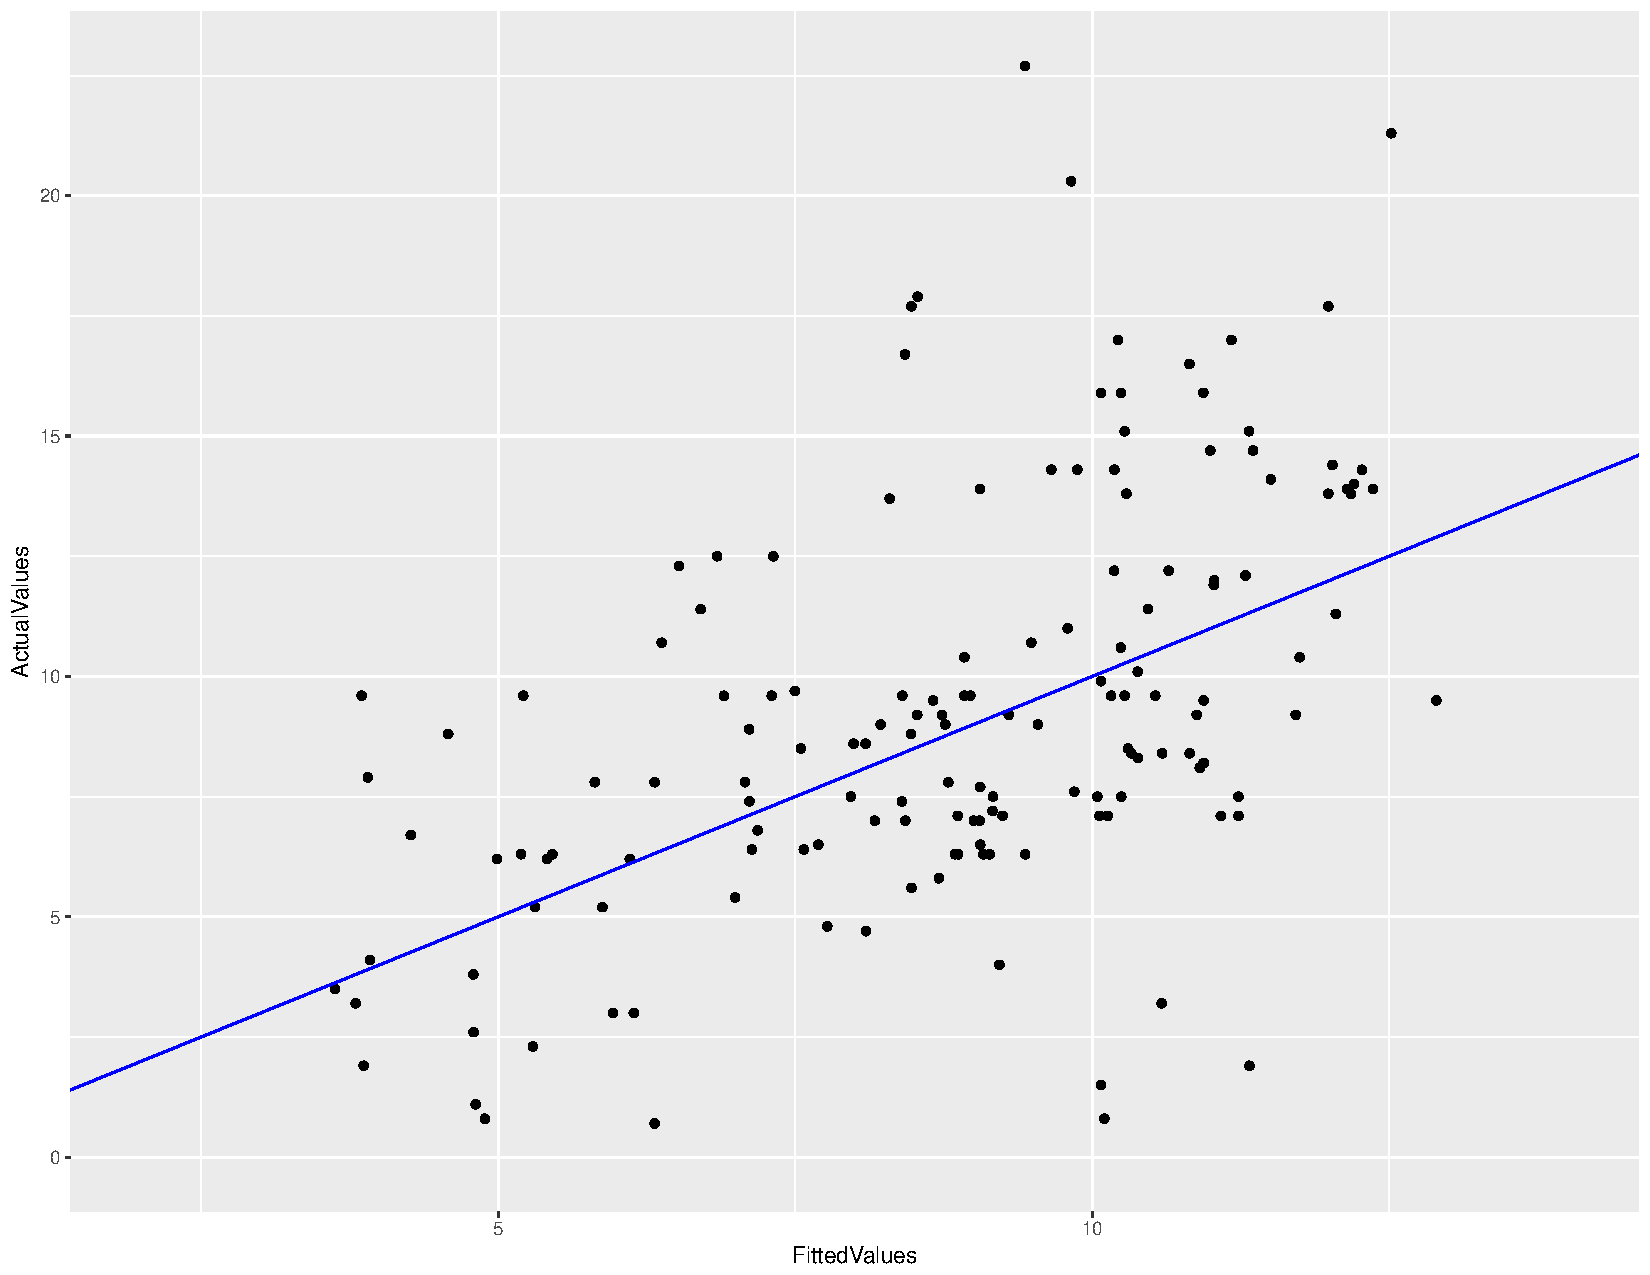
\includegraphics[width=\textwidth]{TestSetFittedVsActual.pdf}
\caption{Test Set Predicted vs Actual ISI}
\label{TestSetPredictedVsActual}
\end{figure}
By considering the predicted ISI values, the mean squared error was calculated to be $13.3$. 
%Fix Up Graphics Path
%\begin{figure}
%\centering
%\includegraphics{FinalModelDiagnostics.pdf}
%\caption{Test Set Diagnostics}
%\label{FinalModelDiagnostics}
%\end{figure}


The analysis on the test set mostly confirms the model selection performed on the training set, with the key difference being the loss of significance for the Is Raining variable.  We conclude that all weather variables except for rain impact the ISI, and fail to conclude that the presence of rain is a predictor for the model. The predictions from the model are reasonably close to the actual data based on an MSE criterion. 




\section{Discussion}\label{Discussion}

\section{Appendix}


\end{document}